\chapter{Introducción}


\section{Fundamentos teóricos de la luz}

\subsection{Radiación electromagnética}

La luz es radiación electromagnética que se propaga en forma de onda a través del espacio transportando energía radiante en el proceso. Está constituida por partículas elementales sin masa denominadas fotones \citep{Purcell&Morin2013}. Las propiedades de la luz están condensadas en el espectro electromagnético (EM) (Figura~\ref{espectroelectromagnetico}) con base en el número de oscilaciones de la onda por unidad de tiempo (frecuencia, $\nu$) y la distancia lineal entre dos puntos equivalentes de ondas sucesivas (longitud de onda, $\lambda$).\\

\begin{figure}
  \centering
    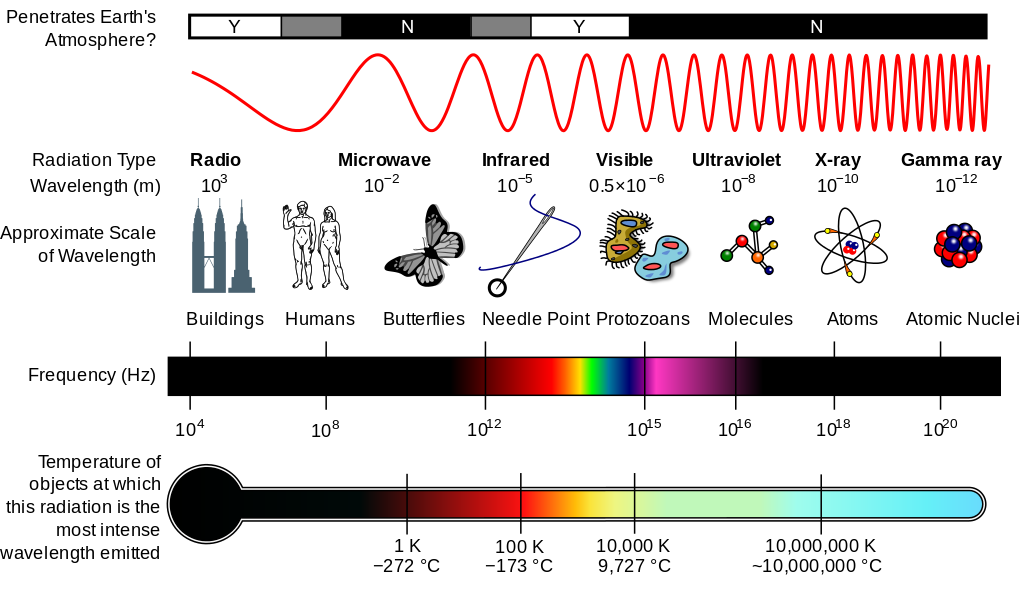
\includegraphics[width=1\textwidth]{espectroelectromagnetico}
  \caption{Espectro electromagnético \citep{NASA2007}}
  \label{espectroelectromagnetico}
\end{figure}

Una de las propiedades de la luz de interés para este trabajo en la región visible del EM ($\sim$ 380-780 nm) es la temperatura de color ($T$)  que está definida a partir de la Ley de desplazamiento de Wien \citep{Halliday&Resnick2008}. Esta ley explica la relación inversa entre la longitud de onda en la que se produce el pico de emisión de un cuerpo negro ($\lambda_{max}$) y $T$:

\begin{equation}
\lambda_{max} = \dfrac{b}{T}
\end{equation}

Donde $b = 2.897...\e{-3}$ m K, es denominada la constante de Wien. Un cuerpo negro es un objeto ideal que absorbe y emite toda radiación electromagnética; en equilibrio termodinámico y térmico, emite radiación térmica sólo con dependencia en su temperatura.\\

En la \textbf{\autoref{sec:luzartificial}} y en la \textbf{\autoref{sec:contaminacionluminica}} se presenta la aplicación del concepto de temperatura de color para la clasificación del color de las fuentes de luz y su implicación biológica en los seres vivos.\\

\subsection{Propiedades ópticas}

La óptica es el campo de la física que se encarga de estudiar la interacción de la luz con la materia. En la  \textbf{Tabla \ref{tab:propiedadesopticas}} se resumen las principales propiedades ópticas.


\begin{table}[htb]
\centering
\tiny
\caption{Propiedades ópticas de la luz  \citep{Born&Wolf2003}}
\label{tab:propiedadesopticas}
\begin{tabular}{lll}
\hline
\textbf{Propiedad} &          & \textbf{Descripción}                             \\ \hline
                                    &          &                                                                         \\
Absorción                           &          & La luz es captada en el objeto y aumenta su energía térmica                       \\
                                    &          &                                                                                   \\
Transmisión                         &          & La luz atraviesa el objeto sin cambio de dirección ni intensidad                  \\
                                    &          &                                                                                   \\
Dispersión                          &          & La luz es captada en el objeto y se re-emite con diferente dirección e intensidad \\
                                    &          &                                                                                   \\
                                    & Rayleigh & Dispersión elástica (conserva energía) en que la longitud de onda de la luz       \\
                                    &          & incidente es mucho mayor que el tamaño del objeto                                 \\
                                    &          &                                                                                   \\
                                    & Mie      & Dispersión elástica en que la longitud de onda de la luz incidente es similar     \\
                                    &          & al tamaño del objeto                                                              \\
                                    &          &                                                                                   \\
Reflexión                           &          & La luz se desvía al chocar con el objeto con un ángulo igual al de incidencia     \\
                                    &          &                                                                                   \\
Refracción                          &          & La luz cambia de dirección y velocidad al atravesar por un medio diferente       
\end{tabular}
\end{table}

\newpage

\subsection{Unidades de medición}

Existen dos campos de estudio que se encargan de la medición de la luz: la fotometría y la radiometría. La fotometría se encarga de medir la luz con base en la sensibilidad de la vista humana. Por otro lado, la radiometría mide la luz abarcando todas las longitudes de onda del EM. Al ser de carácter general este trabajo, en la \textbf{Tabla \ref{tab:unidadesradiometria}} se muestran las unidades del Sistema Internacional de Unidades (SI) utilizadas en radiometría.\\

Para estudios enfocados en los niveles de luminosidad en ecosistemas y su influencia en cada uno de sus componentes con base en su sensibilidad, es fundamental utilizar medidas fotométricas tal y como se aborda en el \textbf{\autoref{chap:recomendaciones}}.


\begin{table}[]
\centering
\caption{Unidades del SI utilizadas en radiometría \citep{Jurgen1968}}
\label{tab:unidadesradiometria}
\resizebox{\textwidth}{!}{
\begin{tabular}{lll}
\hline
\textbf{Magnitud física}            & \textbf{Unidad del SI}                      & \textbf{Notas}                                                    \\ \hline
                                    &                                             &                                                                   \\
Energía radiante (Q)                & julio (J)                                   & Energía                                                           \\
                                    &                                             &                                                                   \\
Flujo radiante ($\Phi$)             & vatio (W)                                   & Energía radiada por unidad de tiempo (potencia)                   \\
                                    &                                             &                                                                   \\
Intensidad radiante (I)             & vatio por estereorradián (W sr$^{-1}$)        & Potencia por ángulo sólido                                        \\
                                    &                                             &                                                                   \\
Irradiancia (E)                     & vatio por metro cuadrado (W m$^{-2}$)         & Potencia incidente por superficie                                 \\
                                    &                                             &                                                                   \\
Emitancia radiante (M)              & vatio por metro cuadrado (W m$^{-2}$)         & Potencia emitida por superficie de la fuente radiante             \\
                                    &                                             &                                                                   \\
Radiancia (L)                       & vatio por estereorradián por metro cuadrado (W sr$^{-1}$  m$^{-2}$) & Potencia por ángulo sólido y por superficie                       \\
                                    &                                             &                                                                   \\
Radiancia espectral ($L_{\lambda}$) & vatio por estereorradián por metro cúbico   (W sr$^{-1}$  m$^{-3}$)   & Potencia por ángulo sólido, por superficie y por longitud de onda
\end{tabular}
}
\end{table}


\section{Brillo del cielo nocturno}

\subsection{Componentes del brillo del cielo nocturno}

En la \textbf{Tabla \ref{tab:componentesbrillo}} se describen los principales componentes del brillo total del cielo nocturno sin Luna $(I_{tot})$ tal como \cite{Leinert1998} lo reportan para el rango del ultravioleta lejano ($\sim$ 100 nm) al infrarrojo lejano ($\sim$ 200 $\mu$m).

\begin{table}[htb]
\centering
\caption{Componentes del brillo del cielo nocturno \citep{Leinert1998}}
\label{tab:componentesbrillo}
\resizebox{\textwidth}{!}{
\begin{tabular}{lllll}
\cline{1-2}
\textbf{Componente} & \textbf{Descripción} &  &  &  \\ \cline{1-2}
 &  &  &  &  \\
Brillo del aire ($I_A$) & Excitación de átomos de oxígeno y nitrógeno de la atmósfera superior por su interacción con la radiación solar &  &  &  \\
 &  &  &  &  \\
Luz zodiacal ($I_{ZL}$) & Dispersión de la radiación solar en partículas de polvo interestelar &  &  &  \\
 &  &  &  &  \\
Luz estelar ($I_{ISL}$) & La luz de las estrellas en su conjunto &  &  &  \\
 &  &  &  &  \\
Luz difusa galáctica ($I_{DGL}$) & Luz emitida y dispersada por partículas de polvo de la galaxia &  &  &  \\
 &  &  &  &  \\
Luz de fondo extragaláctica ($I_{EBL}$) & Luz producida por galaxias o cúmulo de galaxias &  &  &  \\
 &  &  &  &  \\
Luz artificial ($I_{SCA}$) & Luz artificial dispersada en la tropósfera &  &  & 
\end{tabular}
}
\end{table}

La suma de tales componentes (excepto luz artificial, netamente de origen antropogénico) se considera de origen natural y es susceptible de ser atenuada por acción de la extinción atmosférica. De acuerdo con esta clasificación, el brillo total del cielo nocturno puede calcularse a partir de la siguiente ecuación:

\begin{equation}
I_{tot} = (I_A + I_{ZL} + I_{ISL} + I_{DGL} + I_{EBL})\:e^{-\tau} + I_{SCA}
\end{equation}

\vspace{2mm} 

Donde $\tau$ es el coeficiente de extinción atmosférica que depende de la longitud de onda, la distancia cenital (la distancia angular del cuerpo celeste con respecto al cenit), la altura sobre el nivel del mar del observador y las condiciones atmosféricas.\\ 

La definición matemática del brillo total del cielo nocturno nos permite inferir que las principales contribuciones se deben al brillo del aire y a la luz zodiacal; estimaciones experimentales confirman este comportamiento reportando mediciones de hasta 10$^{-4}$ W sr$^{-1}$  m$^{-2}$ atribuibles al brillo del aire \citep{Leinert1998}.\\ 

\subsection{Variación natural del brillo del cielo nocturno por influencia de la Luna}

La luz lunar percibida en la Tierra es resultado de la reflexión de la luz solar y, en menor medida, terrestre en la superficie de la Luna. El albedo lunar es 0.136 lo que significa que refleja 13.6\% del total de la radiación incidente \citep{Matthews2008}. La cantidad de luz lunar varía hasta en tres órdenes de magnitud a lo largo del mes de acuerdo con el ciclo lunar \citep{Kyba2017}.\\

En condiciones atmosféricas despejadas y de nula luz artificial, la luz lunar es la principal responsable del brillo total del cielo nocturno ya que, típicamente, los valores de brillo del aire son hasta tres órdenes de magnitud más pequeños que los reportados para la luz lunar \citep{Hanel2018}.\\

Es importante tomar en cuenta la advertencia de \cite{Kyba2017} quienes reportan que en la literatura científica existen datos erróneos de luz lunar y hacen visible la necesidad de una publicación que reporte valores típicos de referencia de luz lunar a través de estudios de largo plazo (al menos de un año) en localidades sin influencia de luz artificial.\\ 

Tomando en cuenta las consideraciones anteriores, para efectos de este estudio centrado en la luz artificial, se procede a despreciar los términos de luz de origen natural en la ecuación de brillo total del cielo nocturno sin Luna, reduciéndose entonces a:

\begin{equation}
I_{tot} = I_{SCA}
\end{equation}

En la \textbf{\autoref{sec:contaminacionluminica}} se aborda la importancia en términos fotométricos de considerar la influencia de la luz lunar en los ecosistemas a diferentes escalas según la sensibilidad de sus componentes.\\

\subsection{Variación natural del brillo artificial del cielo nocturno por influencia de las condiciones atmosféricas}

En esta sección se presentan los principales mecanismos que dispersan la luz artificial en la tropósfera ($\sim$ 0 - 12 km) \citep{Lohmann2016}.

\subsubsection{Propiedades ópticas del aerosol atmosférico}

La concentración de aerosol atmosférico depende principalmente de emisiones naturales y antropogénicas, patrones de circulación sinóptica, meteorología local y características topográficas \citep{Carabali2017}.\\

\cite{Garstang1991} predijo por primera vez la dispersión de la luz artificial por acción del aerosol atmosférico. Posteriormente \cite{Kocifaj2007} verifica que el aerosol atmosférico puede amplificar o reducir el brillo del cielo nocturno con base en las propiedades ópticas de bulto descritas a continuación.\\

\textit{\textbf{Espesor óptico de aerosol (AOD)}}\\

El AOD es una cantidad adimensional que representa la extinción atmosférica de la luz por el aerosol atmosférico integrada verticalmente en toda la columna atmosférica. La diferencia de potencial ($V$) medido por un fotómetro solar es proporcional a la radiancia espectral ($L_{\lambda}$) que es captada por el instrumento en la superficie \citep{Holben1998}. El espesor óptico total ($\tau_{TOT}$) puede calcularse a partir de la siguiente ecuación conocida como la ley de Beer-Lambert-Bouguer:

\begin{equation}
V(\lambda) = V_0(\lambda)\:d^{2} \:e^{-\tau_{TOT}\: m}
\end{equation}

Donde $V$ es la diferencia potencial medida en una longitud de onda dada $\lambda$, $d$ es la tasa entre el promedio y la distancia real Tierra-Sol y $m$ es la masa óptica de aire. La masa óptica de aire es la tasa entre la masa de aire que la luz solar atraviesa hasta la superficie de la Tierra y la masa de aire que atravesaría si la incidencia fuera vertical.\\

Otros constituyentes atmosféricos pueden dispersar la luz y, por lo tanto, deben de considerarse en el cálculo del AOD \citep{Holben1998} tal y como se muestra en la siguiente ecuación:

\begin{equation}
\tau (\lambda)_{Aerosol} = \tau (\lambda)_{TOT} - \tau (\lambda)_{agua} - \tau (\lambda)_{Rayleigh} - \tau (\lambda)_{O_3} - \tau (\lambda)_{NO_2} - \tau (\lambda)_{CO_2} - \tau (\lambda)_{CH_4}
\end{equation}

\newpage

\textit{\textbf{Parámetro de Angstrom}}\\

La distribución por tamaño del aerosol atmosférico puede ser estimada a través del Parámetro de Amstrong $(\alpha)$ \citep{Holben1998} definido a partir de la siguiente ecuación:

\begin{equation}
\alpha (\lambda_1, \lambda_2) = \frac { -ln (\frac{\tau_\lambda_2}{\tau_\lambda_1})}{ ln(\frac{\lambda_2}{\lambda_1})}
\end{equation}

Donde $\tau_\lambda_1$ y $\tau_\lambda_2$ son el AOD en las longitudes de onda $\lambda_1$ y $\lambda_2$ respectivamente. $\alpha$ $>$ 1, indica que el modo fino de aerosol atmosférico es dominante mientras que  $\alpha$ $<$ 1 indica que el modo grueso es el más abundante \citep{Carabali2017}.\\

\textit{\textbf{Parámetro de Asimetría (ASY)}}\\

Definido como el promedio del coseno del ángulo de dispersión ponderado por intensidad. Su valor es una medida de la dirección de la dispersión de la luz. Cuando ASY = 1, toda la luz es dispersada hacia adelante; ASY = 0, indica una dispersión isotrópica \citep{Solano2015}.\\

\textit{\textbf{Albedo de Dispersión Simple (SSA)}}\\

Este parámetro relaciona los coeficientes de dispersión ($\epsilon_{SCA}$) y absorción ($\epsilon_{ABS}$) \citep{Foot1987} como muestra la ecuación:

\begin{equation}
SSA = \frac{\epsilon_{SCA}}{\epsilon_{SCA} + \epsilon_{ABS}}
\end{equation}

De esta definición se puede inferir que para el aerosol atmosférico que menos absorbe, el valor del SSA es cercano a 1, mientras que, para el menos absorbentes, el valor de SSA es cercano a 0.\\

\subsubsection{Propiedades ópticas de las nubes}

\cite{Twomey1967} desarrolló por primera vez una teoría de dispersión de la luz debido a la nubosidad. Estudios más recientes \citep{Kocifaj2007}, \citep{Solano2014}, \citep{Solano2015}, han encontrado cambios significativos en el brillo del cielo por la dispersión de luz artificial por acción de la nubosidad. Las nubes son un medio dispersivo complejo, esto es, que poseen diferentes constituyentes con diferente índice refractivo complejo $(\underline{n})$ definido como:

\begin{equation}
\underline{n} = n + i k
\end{equation}

\vspace{2mm} 

Donde $n$, la parte real de la ecuación, indica la velocidad de la luz dentro de un medio y la parte imaginaria $k$ es el coeficiente de extinción, una medida de la atenuación de la luz dentro del medio en cuestión \citep{Born&Wolf2003}. Los valores de la parte imaginaria del índice refractivo complejo para las gotitas de nube y los cristales de hielo que forman las nubes son muy bajos de acuerdo con \cite{Solano2015}.\\

Tomando en cuenta lo anterior, \cite{Solano2015} consideran a las nubes como cuerpos Lambertianos con albedo espectral variante para su estudio óptico. Un cuerpo Lambertiano es aquel que posee una superficie ideal que refleja la luz incidente de manera isotrópica, permitiendo así que el brillo de tal superficie sea la misma para el observador independientemente de su ángulo de visión \citep{Born&Wolf2003}.\\

El albedo espectral de las nubes depende principalmente de factores como la altitud de su base con respecto al observador y la microfísica incluyendo el contenido de agua líquida y la distribución por tamaño de las gotitas de nube \citep{Kocifaj2007}.\\ 

Resulta complicado medir el albedo espectral de las nubes durante la noche ya que la mayoría de los fotómetros que miden esta propiedad funcionan con base en niveles de radiación presentes sólo durante el día. Por esta razón, las simulaciones numéricas de la influencia de las nubes en el brillo del cielo nocturna resultan útiles \citep{Solano2015}.\\

Además, es importante mencionar que los factores que se toman en cuenta en la modelación teórica son capaces de reproducir diferentes comportamientos del brillo del cielo con respecto a la posición del observador, lo cual es deseable para la predicción del brillo del cielo nocturno influenciado por diferentes tipos de nubes \citep{Kocifaj2007}, \citep{Solano2015}.

\newpage

\section{Luz artificial}\\
\label{sec:luzartificial}

En esta sección se aborda la caracterización de la luz artificial (de origen netamente antropogénico). Para esta tesis se considera que el alumbrado público es el principal responsable del brillo del cielo nocturno por luz artificial \citep{Solano2013b}.

\subsection{Fundamentos teóricos de las fuentes artificiales de luz}

El diseño de iluminación es una disciplina fundamental para la correcta iluminación en el alumbrado público, la cual requiere de colaboraciones con otros campos como la física, biología, ciencias de la Tierra, ingeniería y arquitectura. El reto es grande ya que una correcta iluminación debe ser sustentable, apropiada para su contexto y debe lograr ahorro económico \citep{LibroCL}, \citep{Globaldiscussion}. A continuación se presentan los conceptos físicos fundamentales detrás de la correcta iluminación.\\


\textit{\textbf{Producción de luz}}

Para la producción artificial de luz se necesita de una serie de transformaciones de energía. El primer paso es la generación de energía eléctrica. De acuerdo con \cite{Ramos2012}, la mayoría de la energía eléctrica consumida en México es generada a partir de la transformación de energía química por medio de la combustión de hidrocarburos.\\

Una vez generada la energía eléctrica, necesita ser transformada en energía radiante. Esto se logra por medio del mecanismo interno de la fuente de luz. Los mecanismos más utilizados son la termorradiación (radiación de un cuerpo caliente) y luminiscencia (radiación de cuerpo no caliente) \citep{LibroCL}. En la \textbf{\autoref{subsec:fuentesdeluz}} se abordan las particularidades de cada uno de estos mecanismos.\\


\textit{\textbf{Distribución espectral}}

La cantidad de energía radiada en determinadas regiones del EM \citep{Solano2013}. En la \textbf{\autoref{subsec:fuentesdeluz}} se muestran los gráficos de distribución espectral para diferentes tipos de fuentes de luz artificial.\\

  
\textit{\textbf{Temperatura de color}}

La temperatura de color define el color de una fuente de luz sólo si esta se asemeja a un cuerpo negro. La mayoría de las fuentes de luz tradicionalmente utilizadas (incandescentes) se asemejan a un cuerpo negro, mientras que para las que no cumplen con esa característica (de descarga y LED), se implementa la temperatura de color correlacionada \citep{LibroCL}.\\

Para efectos de evaluación de reproducción de color y confort se asocia una apariencia de color a los rangos de temperatura de color teniendo <<luz cálida>> para temperatura de color de hasta 3000 K, <<luz intermedia>> de 3000 - 5300 K y <<luz fría>> para temperaturas de color mayor a 5300 K \citep{Globaldiscussion}.\\


\textit{\textbf{Eficiencia}}

Definida para estudios fotométricos, se trata de la cantidad de flujo luminoso (visible) emitido por una fuente de luz por unidad de potencia consumida. La unidad del flujo luminoso es el lumen (lm), el equivalente fotométrico del flujo radiante. No es posible obtener una eficiencia de 100$\%$ debido a las pérdidas ocasionadas por disipación calorífica y radiaciones no visibles para el humano \citep{LibroCL}.


\subsection{Fuentes de luz artificial}
\label{subsec:fuentesdeluz}

Existen tres principales tipos de fuentes de luz artificial: incandescente, de descarga y diodo emisor de luz (LED, por sus siglas en inglés) \citep{Solano2013b}, \citep{Eldvidge2010}, \citep{LibroCL}.\\

La iluminación incandescente es la más antigua y la más utilizada para interiores, su funcionamiento se basa en hacer pasar corriente eléctrica a través de un filamento, aumentando su temperatura hasta hacer que emita radiaciones visibles (termorradiación).\\

Por otro lado, la luz de descarga, utilizada ampliamente para alumbrado público, es generada por la excitación de un gas sometido a descargas eléctricas entre dos electrodos (luminiscencia).\\

Por último, el LED, que recientemente se ha comenzando a implementar en el alumbrado público, genera luz moviendo electrones de un semi-conductor sólido de un estado de alto nivel de energía a uno más bajo a través de la aplicación de una diferencia de potencial (electroluminiscencia).\\

 En la \textbf{Tabla \ref{tab:luzartificial}} se presentan ejemplos de las principales fuentes de luz artificial. 


\begin{table}[htb]
\tiny
\centering
\caption{Principales fuentes de luz artificial \citep{Solano2013b}, \citep{Eldvidge2010}, \citep{LibroCL}}
\label{tab:luzartificial}
\begin{tabular}{llllll}
\hline
\textbf{Tipo} & \textbf{Fuente de luz} & \textbf{Distribución espectral (ver Figura~\ref{distribucionespectral})} & \textbf{Temperatura de color (K)} & \textbf{Eficiencia (lm W$^{-1}$}) \\ \hline
 &  &  &  &  &  \\
Incandescente & Lámpara incandescente & Continuo en el visible & 2700 & 8 - 18 (baja)\\
 &  &  &  &  &  \\
 & Lámpara de sodio a baja presión (LPS) & Discontinuo con pico en 589 nm & 2000 & 180 (muy alta)\\
 &  &  &  &  &  \\
 & Lámpara de sodio a alta presión (HPS) & Discontinuo con pico en 819 nm & 2300 & 100 (alta)\\
De descarga &  &  &  &  &  \\
 & Lámpara de halogenuros metálicos (MH) & Discontinuo con pico alrededor de 600 nm y en 819 nm & 2800 - 5000 & 70 - 90 (alta)\\
 &  &  &  &  &  \\
 & Lámpara de vapor de mercurio (MV) & Discontinuo con picos en 546 y 578 nm & 3200 - 4000 & 60 (media)\\
 &  &  &  &  &  \\
LED & LED & Continuo en el visible & 2700 - 5000 & 10 - 150 (baja)\\
 &  &  &  &  & 
\end{tabular}
\end{table}

\begin{figure}[htb]
  \centering
    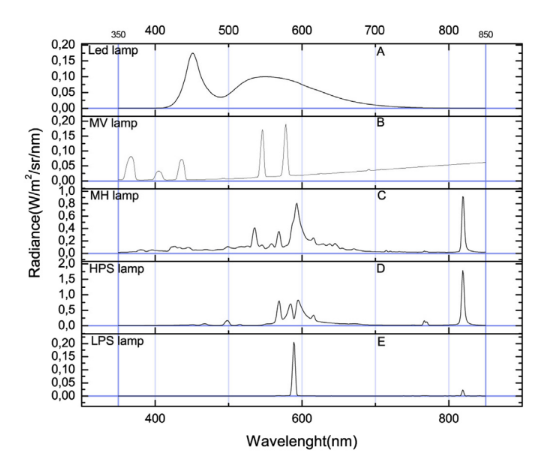
\includegraphics[width=70mm, scale=0.7]{distribucionespectral}
  \caption{Distribución espectral de A) LED, B) Vapor de mercurio, C) Halogenuros metálicos, D) Sodio a alta presión y E) Sodio a baja presión \citep{Solano2013b}}
  \label{distribucionespectral}
\end{figure}

\newpage

\subsection{Tipos de luminarias}

Las luminarias son dispositivos que alojan y protegen la fuente de luz y reconducen su luz hacia donde se quiere iluminar \citep{LibroCL}. Para el caso del alumbrado público existen dos tipos: luminarias para vías principales (autopistas, carreteras) y luminarias para vías secundarias (calles) \citep{INFO2019}.\\

La forma en que la luminaria distribuye en el espacio la luz emitida por la fuente es fundamental en el efecto sobre el brillo del cielo nocturno. \cite{Marin2009} propone el ángulo entre la línea vertical de la fuente de luz y la línea máxima a la que ilumina (ángulo de apantallamiento) para garantizar un buen aprovechamiento de la luz y evitar que se desperdicie escapando hacia la atmósfera. El ángulo de apantallamiento ideal es por debajo de los 75\grad (A); para ángulos mayores a ese (B - E) existe afectación en diferente proporción al brillo del cielo nocturno (Figura~\ref{anguloapantallamiento}).


\begin{figure}[htb]
  \centering
    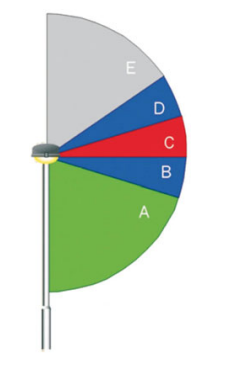
\includegraphics[width=30mm, scale=0.3]{anguloapantallamiento}
  \caption{Ángulo de apantallamiento de luminaria \citep{Marin2009}}
  \label{anguloapantallamiento}
\end{figure}


\subsection{Función de emisión urbana}

La distribución angular de la luz emitida por una ciudad es fundamental para la modelación del brillo del cielo nocturno ocasionado por luz artificial \citep{Kocifaj2014}.\\

Las fuentes de luz artificiales (públicas y privadas) emiten luz en casi todas las direcciones \citep{Kocifaj2014}, \citep{Kocifaj2016}. Por lo tanto, la luz artificial emitida a la atmósfera se debe a la superposición de emisiones de las diferentes fuentes distribuidas en la superficie.\\

La luz emitida por una región (o incluso a nivel fuente puntual) es caracterizada a través de una función de emisión parametrizada denominada Función de Emisión Urbana (CEF, por sus siglas en inglés) la cual únicamente depende de las características del sistema de iluminación de una ciudad \citep{Kocifaj2014}.\\

Debido a la falta, hasta la actualidad, de inventarios detallados de las fuentes de luz (públicas y privadas) y su naturaleza heterogénea, resulta extremadamente complicado obtener la CEF a través de estudios teóricos o experimentales \citep{Kocifaj2014}. \cite{Garstang1986} desarolló una aproximación semi-empírica para la estimación de la CEF basándose en datos poblacionales (emisiones de luz per cápita) que es ampliamente utilizada hoy en día.

\newpage

\section{Contaminación lumínica (CL)}\\
\label{sec:contaminacionluminica}

La CL es el conjunto de efectos de difusión, en la atmósfera nocturna, de la luz producida por fuentes artificiales que alteran las condiciones originales de luminosidad; estos efectos se producen por la emisión del flujo luminoso en intensidades, direcciones, rangos espectrales u horarios innecesarios \citep{AtlasREPSA}, \citep{LibroCL}, \citep{Stone2017}.\\

En esta sección se presentan los argumentos que permiten afirmar que el brillo del cielo nocturno debido a la luz artificial, discutido en secciones anteriores, es una fuente de contaminación en los socioecosistemas.\\

Para efectos del presente trabajo entiéndase un sistema como un conjunto de componentes interactuando en los que: 1) el comportamiento de cada componente tiene un efecto en el comportamiento del todo y, 2) el comportamiento de los componentes y sus efectos en el todo son interdependientes \citep{Avila2019}.\\

\subsection{El enfoque socioecosistémico}

Los seres humanos nombramos a la realidad natural de distintas maneras, las cuales poseen significados brutalmente diferentes de acuerdo con el fundamento filosófico con el que percibimos el planeta \citep{Avila2019}, \citep{Uribe2014}. Por ejemplo, las empresas extractivas denominan <<recursos naturales>> a tal realidad, los habitantes de una región, <<territorio>> y los científicos, <<ecosistema>>.\\

Con la aparición de la vida en la Tierra, surgieron los ecosistemas como un nivel de organización de la materia y la energía, en que el los sistemas físico-químicos (abióticos) y los sistemas bióticos interctuaron y evolucionaron de manera integrada. Sin embargo, con la emergencia de las sociedades humanas y su organización con base en un lenguaje simbólico, nacen los socioecosistemas \citep{Avila2019}, \citep{Uribe2014}, \citep{Urquiza2015}.\\

Un socioecosistema es, por lo tanto, un sistema complejo (no lineal) y adaptativo que hace referencia a los procesos de acoplamiento e interacción entre los sistemas sociales (cultura, economía, organización social y política) y los ecosistemas \citep{Urquiza2015}.\\

Resulta fundamental, entonces, estudiar las problemáticas de contaminación ambiental desde el enfoque socioecosistémico. De esta manera se hace visible que, separar el nicho humano de la realidad natural, es el principal motor de la actual crisis ambiental. En este sentido, las Ciencias de la Tierra surgen como la disciplina integradora que, a través de la generación de conocimiento con un enfoque socioecosistémico, logra sembrar directrices en la construcción de la sustentabilidad.\\

\subsection{Importancia del ciclo día-noche en la evolución de la vida}

La duración del ciclo día-noche en la Tierra ha cambiado significativamente a lo largo de la historia geológica debido a la variación de la velocidad de rotación del planeta. La velocidad de rotación original de los planetas  es consecuencia de la conservación del momento angular que poseía la nebulosa interestelar que, al colapsar, dio origen al Sistema Solar hace aproximadamente 4600 Ma \citep{Greaves2005}.\\

Sin embargo, si la hipótesis del Impacto de Theia es correcta, es factible que la rotación primordial de la Tierra haya sido reconfigurada hace alrededor de 4500 Ma, cuando un cuerpo astronómico del tamaño de Marte, nombrado Theia, colisionó tangencialmente con nuestro planeta dando origen, además, a la Luna \citep{Stevenson1987}.\\

La velocidad de rotación actual de la Tierra debió comenzarse a perfilar hacia finales del periodo Criogénico (hace alrededor de 600 Ma), al mismo tiempo que los niveles de oxígeno y ozono estratosférico fueron óptimos para el surgimiento y desarrollo de vida más compleja (multicelular) en un evento conocido como \textit{la Radiación del Cámbrico}, durante el que se originaron y diversificaron la mayoría de los filos animales incluyendo el de los cordados, al que pertenecemos los humanos \citep{Conway2000}.\\

La mayoría de los organismos, incluyendo a los humanos, poseen ritmos circadianos que son controlados por el ciclo día-noche. Tales ritmos juegan un papel primordial en la regulación del metabolismo, el crecimiento y el comportamiento \citep{Dunlap1999}. Los fotoreceptores circadianos han estado presentes en la retina de los vertebrados desde hace aproximadamente 500 Ma, una vez que la duración del día se estableció en 24 horas \citep{Conway2000}, \citep{Longcore2006}.
\\

Se ha encontrado que la proporción de especies vertebradas nocturnas que surgieron durante radiaciones evolutivas recientes es mayor con respecto a las antiguas (Figura~\ref{nocturnalidad}). Esto sugiere que la nocturnalidad es un importante paso en la evolución de los vertebrados \citep{Holker2010}.\\

Se teoriza que dada la alta permeabilidad de la piel de los anfibios y por ende, la susceptibilidad a las características de los nichos diurnos como la radiación solar, estos tuvieron que adoptar la nocturnalidad tempranamente \citep{Holker2010}.\\

\begin{figure}[htb]
  \centering
    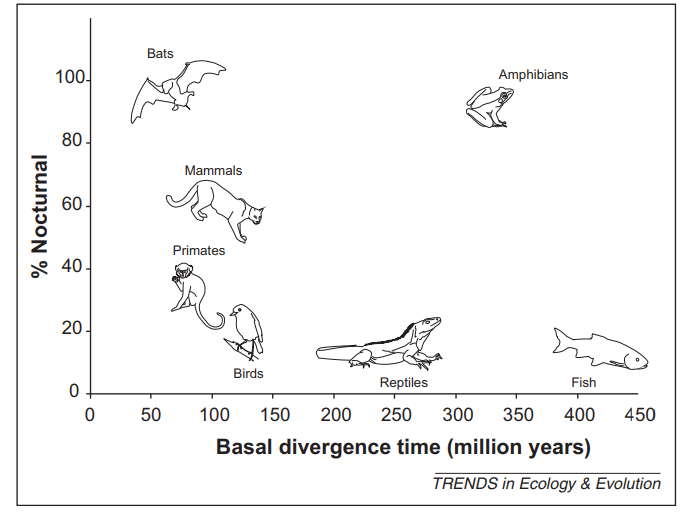
\includegraphics[width=80mm, scale=0.8]{nocturnalidad}
  \caption{Porcentaje de especies nocturnas de diferentes clases y órdenes de vertebrados con respecto a su origen \citep{Holker2010}}
  \label{nocturnalidad}
\end{figure}

 No sólo la nocturnalidad es importante en los vertebrados. Se estima que más del 60$\%$ de invertebrados son nocturnos \citep{Longcore2006}.\\

\subsection{Historia del uso y abuso de la luz}

Embers of society, revolución industrial, capitalismo. tendencias mundiales 

Conclusión: la CL es producida por una visión no sustentable de los "recursos".

\subsection{Tipos de CL} 

Aunque sólo se ha discutido el brillo del cielo nocturno, hay otros tipos de CL que es importante mencionar. 

\subsection{Consecuencias de la CL}

PRIMARIAS

En qué región del espectro se ven afectadas diferentes clases de animales de acuerdo con su visión (luminancia).\\

SECUNDARIAS

Podrían estimular la nucleación de partículas ultrafinas que se forman por reacciones fotoquímicas.

Calentamiento global 

\subsection{Contexto histórico del estudio de la CL}

Revisión de la tesis de Héctor Linares

On the relation between zenith sky brightness andhorizontal illuminance

Modelo teórico vs medidas experimantales con SQM, Por qué utilizar modelos en vez de mediciones puntuales.

\subsection{Marco regulatorio: normas y leyes en México y el mundo}

PREOCUPACIÓN POR QUE LA LEGISLACIÓN FEDERAL SEA SUSTENTABLE Y CON BASES CIENTÍFICAS Y ESTUDIOS.

Ley 31/1998 Protección de la Calidad Astronómica de los Observatorios del Instituto de Astrofísica de Canarias.\\

Ley 6/2001 Ordenación ambiental del alumbrado para la protección del medio nocturno.\\

Zonificación con 4 categorías y una especial.\\

\begin{itemize}

    \item E1. Espacios que por sus características naturales o su valor astronómico especial, sólo se puede admitir un brillo mínimo.
    
    \item E2. Áreas incluidas en ámbitos territoriales que sólo admiten un brillo reducido.
    
    \item E3. Áreas incluidas en ámbitos territoriales que admiten un brillo medio
    
    \item E4. Áreas incluidad en ámbitos territoriales que admiten un brillo alto.
    
    \item Puntoa de referencia. Puntos cercanos a las áreas de valor astronómico o natural especial incluidos en E1, para los que hay que establecer una regulación específica en función de la distancia a la que se encuentren del área en cuestión.
    
    
\end{itemize}

Según el Departamento de Estudios Luminotécnicos de la ETSEIB (UPC) en \textit{Evaluación del Impacto Ambiental Lumínico en Zonas Protegidas del Área Metropolitana de Barcelona}, los aspectos importantes para controlar la Contaminación Lumínica son:

\begin{itemize}
    \item Niveles más estrictos a los permisos de las luminarias (Comité Internationale d'Eclairage)
    
    \item Límites de luminosidad en el espacio-tiempo (periodo de protección especial a partir de las 23 hrs.)
    
     \item Cambiar el uso de luz blanca (especialmente nociva) a una temperatura de color neutra (4200 K), promoviendo las cálidas (inferiores a 3000 K)
     
\end{itemize}


\section{Estudio de caso: Ciudad de México}

Revisión de Tweets

\subsection{Descripción del área de estudio}

División política, extensión, situación geográfica, 

Incluir REPSA

\subsection{Inventario de alumbrado público}

Incluir número total de luminarias

\subsection{Consumo de energía eléctrica}

Datos de consumo de energía eléctrica por entidad federativa por el Sistema de Información Energética de la Secretaría de Energía.\\

Su relación con las emisiones de gases de efecto invernadero 

\subsection{Climatología de aerosol atmosférico y nubosidad}

Artículo de Giovanni Caraballi

Mexico City is located in a sub-tropical zone where the seasons can
be generally separated into three periods (Jáuregui, 2002; de Foy et al.,
2005; Collins and Scott, 1993): the Dry Winter (DW) season from
November to March, the Dry Spring (DS) season from April through
May, and the RAiny (RA) season from June until October. The starting
and ending dates for these seasons vary from year to year, but these

three seasonal periods will be employed in the analysis as an opera-
tional definition,

Qué nubes son típicas en cada estación del año: hurcanes vs frentes fríos

\section{Hipótesis}

\section{Objetivos}

\subsection{Generales}

\begin{itemize}

    \item Reproducir el modelo \textit{SkyGlow} para el caso de la Ciudad de México
    
    \item Estimar los niveles de contaminación lumínica en la Ciudad de México 
    
    \item Generar un antecedente para la campaña de validación del modelo \textit{SkyGlow} en la Ciudad de México
    
\end{itemize}

\subsection{Particulares}

\begin{itemize}

    \item Caracterizar el alumbrado público de la Ciudad de México 
    
    \item Elaborar un mapa teórico de contaminación lumínica de la Ciudad de México bajo condiciones de cielo despejado
    
    \item Construir mediante simulaciones diferentes escenarios del brillo del cielo nocturno tomando en cuenta diferentes posiciones del observador y condiciones atmosféricas
    
    \item Inferir la influencia del aerosol atmosférico  y la nubosidad en el brillo del cielo nocturno a partir del objetivo anterior
    
    
\end{itemize}